\vspace*{3cm}
\noindent \textbf{\Huge Chapitre 7} \\[1cm]  % Large title for the chapter
\textbf{\Huge Classification des états} \\[1.5cm]  % Sub-title

\section{Classification des états}
\thispagestyle{plain} % First page of the chapter with no header
\fancyhead[R]{\textbf{Chapitre 7. Classification des états}} % Set custom header title
L’espace des états étant souvent de grande taille, il est utile de le partitionner en des sous-ensembles dont les éléments ont les mêmes comportements au regard de propriétés importantes. Pour ce faire, nous introduisons une relation d’équivalence sur les états.

\subsection{Classes de communication}
On considère une chaîne de Markov $(X_n)_{n \geq 0}$ définie sur un espace d’états $E$, de matrice de transition $P$.

\begin{definition}[7.1]

\begin{itemize}
    \item Soient deux états $x$ et $y$. Nous dirons que $x$ conduit à $y$ ou que $y$ est accessible depuis $x$, noté $x \to y$, si :
    \[
    \exists n \in \mathbb{N},\ P^{(n)}(x, y) = P[X_n = y \mid X_0 = x] > 0.
    \]
    Cette relation signifie que partant de $x$, nous avons une probabilité non nulle d’atteindre $y$ à un certain temps $n$.

    \item Nous dirons que $x$ communique avec $y$, noté $x \leftrightarrow y$, si chacun des états $x$, $y$ est accessible depuis l’autre, c’est-à-dire $x \to y$ et $y \to x$.
\end{itemize}
\end{definition}



\begin{proposition}
La relation de communication $\leftrightarrow$ est une relation d’équivalence.
\end{proposition}

\begin{proof}
\begin{itemize}
    \item \textbf{Réflexivité}: $x \leftrightarrow x$. Immédiat en observant que 
    \[
    P^{(0)}(x, x) = P[X_0 = x \mid X_0 = x] = 1.
    \]

    \item \textbf{Symétrie}: $x \leftrightarrow y \implies y \leftrightarrow x$. Évident par définition.

    \item \textbf{Transitivité}: $x \leftrightarrow y$ et $y \leftrightarrow z \implies x \leftrightarrow z$. Pour cela, il suffit de montrer la transitivité de la relation d’accessibilité. Supposons que $x \to y$ et $y \to z$. Alors il existe $m, n \in \mathbb{N}$ tels que $P^{(n)}(x, y) > 0$ et $P^{(m)}(y, z) > 0$. Or, d’après les équations de Chapman-Kolmogorov, on a 
    \[
    P^{(n+m)}(x, z) = \sum_{y' \in E} P^{(n)}(x, y')P^{(m)}(y', z) \geq P^{(n)}(x, y)P^{(m)}(y, z) > 0.
    \]
    La première inégalité provient du fait que tous les termes de la somme sont positifs ou nuls. En conséquence, $x \to z$.
\end{itemize}
\end{proof}


\begin{definition}[7.3]
\begin{itemize}
    \item Les états $E$ de la chaîne peuvent être partitionnés en classes d’équivalence appelées \textbf{classes irréductibles}. Si $E$ est réduit à une seule classe, la chaîne de Markov est dite \textbf{irréductible}.

    \item La relation d’accessibilité s’étend aux classes : une classe d’équivalence $C'$ est accessible depuis une classe $C$, noté $C \to C'$, si 
    \[
    \forall (x, x') \in C \times C',\ x \to x'.
    \]
    À noter l’équivalence :
    \[
    \forall (x, x') \in C \times C',\ x \to x' \iff \exists (x, x') \in C \times C',\ x \to x'.
    \]
    La relation d’accessibilité définit une relation d’ordre partiel entre les classes d’équivalence.

    \item Une classe d’équivalence $C$ est dite \textbf{fermée} si, pour tout $x, y$ tels que $(x \in C$ et $x \to y \implies y \in C)$. Autrement dit, $\forall x \in C$, $\forall n \in \mathbb{N}$, 
    \[
    \sum_{y \in C} P^{(n)}(x, y) = 1,
    \]
    autrement dit encore, $C$ est une classe dont on ne peut pas sortir.

    \item Une classe fermée réduite à un point $C = \{x\}$ est appelée un \textbf{état absorbant}. Un état $x$ est absorbant si et seulement si $p(x, x) = 1$.
\end{itemize}
\end{definition}


\subsection{Période}
Dans cette partie, nous étudions la période associée à une classe.

\begin{definition}[7.4]
Étant donné un état $x \in E$, la période de l’état $x$, notée $d(x)$, est le plus grand commun diviseur des entiers $n$ tels que $P^{(n)}(x, x)$ est strictement positif :
\[
d(x) = \mathrm{PGCD}\{n \geq 1 \mid P^{(n)}(x, x) > 0\}.
\]
Par convention, $d(x) = 0$ si l’ensemble des $n \geq 1$ tels que $P^{(n)}(x, x) > 0$ est vide.
\end{definition}

\begin{theorem}[7.5]
Si deux états communiquent, alors ils ont la même période.
\end{theorem}

\begin{proof}
Soient $x$ et $y$ deux états qui communiquent, $x \leftrightarrow y$. Montrons que $d(y)$ divise $d(x)$. Ceci revient à prouver que $d(y)$ divise tout $n \geq 1$ tel que $P^{(n)}(x, x) > 0$ ; soit donc un tel $n$. Comme $x$ et $y$ communiquent, il existe deux entiers $k, \ell \geq 1$ tels que $P^{(k)}(x, y) > 0$ et $P^{(\ell)}(y, x) > 0$. De plus, d’après les équations de Chapman-Kolmogorov :
\[
P^{(n+k+\ell)}(y, y) \geq P^{(\ell)}(y, x)P^{(n)}(x, x)P^{(k)}(x, y) > 0, 
\]
et 
\[
P^{(k+\ell)}(y, y) \geq P^{(\ell)}(y, x)P^{(k)}(x, y) > 0.
\]
Ainsi, $d(y)$ divise $n + k + \ell$ et $k + \ell$ ; et par suite, divise la différence $n$. On a donc montré que $d(y)$ divise $d(x)$. En intervertissant les rôles de $x$ et $y$, nous prouvons que $d(x)$ divise $d(y)$, ce qui entraîne que $d(x) = d(y)$.
\end{proof}

\begin{definition}[7.6]
La période d’une classe est la période de chacun de ses éléments. Une classe est dite \textbf{apériodique} si sa période est 1.
\end{definition}


\subsection{Exercices : Classes de communication et période}
%\begin{exercise}[7.1]
\begin{exercise}[7.3]
Considérons une chaîne de Markov définie sur un espace $E = \{0, \dots, 9\}$ formé de 10 états, dont la matrice de transition est :

\[
P =
\begin{pmatrix}
0 & 0.7 & 0 & 0 & 0.3 & 0 & 0 & 0 & 0 & 0 \\
0 & 0 & 1 & 0 & 0 & 0 & 0 & 0 & 0 & 0 \\
0 & 0 & 0 & 1 & 0 & 0 & 0 & 0 & 0 & 0 \\
1 & 0 & 0 & 0 & 0 & 0 & 0 & 0 & 0 & 0 \\
0 & 0 & 0 & 0 & 0 & 1 & 0 & 0 & 0 & 0 \\
0 & 0 & 0 & 0 & 0 & 0 & 1 & 0 & 0 & 0 \\
0 & 0 & 0 & 0 & 0 & 0 & 0 & 1 & 0 & 0 \\
0 & 0 & 0 & 0 & 0 & 0 & 0 & 0 & 1 & 0 \\
0 & 0 & 0 & 0 & 0 & 0 & 0 & 0 & 0 & 1 \\
1 & 0 & 0 & 0 & 0 & 0 & 0 & 0 & 0 & 0
\end{pmatrix}.
\]

\begin{enumerate}
    \item \textbf{Tracer son graphe.}
    \item \textbf{Déterminer les classes de la chaîne et leurs périodes.}
\end{enumerate}
\end{exercise}

\subsection*{Solution de l’exercice 7.1}
\begin{enumerate}
    \item Traçons son graphe :

    \begin{figure}[h!]
    \centering
    \begin{tikzpicture}[>=stealth, node distance=2cm]

        % Styles for nodes and groups
        \tikzstyle{state} = [circle, draw, fill=red!40, minimum size=0.8cm]
        
        % Nodes
        \node[state] (0) {0};
        \node[state] (1) [below left=0.5cm and 0.7cm of 0] {1};
        \node[state] (2) [left=2cm of 0] {2};
        \node[state] (3) [above left=0.5cm and 0.7cm of 0] {3};
        \node[state] (4) [above right=0.5cm and 0.5cm of 0] {4};
        \node[state] (5) [right=1cm of 4] {5};
        \node[state] (6) [right=1cm of 5] {6};
        \node[state] (9) [below right=0.5cm and 0.5cm of 0] {9};
        \node[state] (8) [right=1cm of 9] {7};
        \node[state] (7) [right=1cm of 8] {7};

        % Arrows
         \draw[->, thick] (0) -- node[right] {0.7} (1);
         \draw[->, thick] (1) -- node[left] {1} (2);   
         \draw[->, thick] (2) -- node[above] {1} (3);
         \draw[->, thick] (3) -- node[above] {1} (0);

         \draw[->, thick] (0) -- node[left] {0.3} (4);
         \draw[->, thick] (4) -- node[above] {1} (5);
         \draw[->, thick] (5) -- node[above] {1} (6);
         \draw[->, thick] (6) -- node[right] {1} (7);
         \draw[->, thick] (7) -- node[below] {1} (8);
         \draw[->, thick] (8) -- node[left] {1} (9);
         \draw[->, thick] (9) -- node[left] {1} (0);
    \end{tikzpicture}
\end{figure} 
    \newpage
    \item Nous constatons qu’il y a deux cycles donc les états de chacun des deux cycles communiquent. De plus, ces deux cycles contiennent le même état $0$, ce qui implique qu’ils communiquent. Il n’y a donc qu’une seule classe ; la chaîne est \textbf{irréductible}.
    
    Afin de déterminer la période de cette chaîne de Markov, il suffit de déterminer celle d’un de ses états ; prenons $x = 0$. Partant de $0$, nous sommes de nouveau en $0$ au bout de $4$ transitions en passant par le petit cycle et au bout de $7$ transitions en passant par le grand cycle. Nous avons :
    \[
    P^{(4)}(0, 0) = 0.7 \quad \text{et} \quad P^{(7)}(0, 0) = 0.3.
    \]
    Nous en déduisons que le PGCD ne peut être que $1$ ; la chaîne est donc \textbf{apériodique}. En résumé, cette chaîne est formée d’une seule classe apériodique.
\end{enumerate}


\begin{exercise}[7.2]
Reprenons la chaîne précédente avec un état de moins dans le second cycle. C’est-à-dire, considérons la chaîne de Markov définie sur un espace $E = \{0, \dots, 8\}$ formé de 9 états, dont la matrice de transition est :

\[
P =
\begin{pmatrix}
0 & 0.7 & 0 & 0 & 0.3 & 0 & 0 & 0 & 0 \\
0 & 0 & 1 & 0 & 0 & 0 & 0 & 0 & 0 \\
0 & 0 & 0 & 1 & 0 & 0 & 0 & 0 & 0 \\
1 & 0 & 0 & 0 & 0 & 0 & 0 & 0 & 0 \\
0 & 0 & 0 & 0 & 0 & 1 & 0 & 0 & 0 \\
0 & 0 & 0 & 0 & 0 & 0 & 1 & 0 & 0 \\
0 & 0 & 0 & 0 & 0 & 0 & 0 & 1 & 0 \\
0 & 0 & 0 & 0 & 0 & 0 & 0 & 0 & 1 \\
1 & 0 & 0 & 0 & 0 & 0 & 0 & 0 & 0
\end{pmatrix}.
\]

\begin{enumerate}
    \item \textbf{Tracer son graphe.}
    \item \textbf{Déterminer les classes de la chaîne et leurs périodes.}
\end{enumerate}
\end{exercise}

\subsection*{Solution de l’exercice 7.2}
\begin{enumerate}
    \item Traçons son graphe :

    \begin{figure}[h!]
    \centering
    \begin{tikzpicture}[>=stealth, node distance=2cm]

        % Styles for nodes and groups
        \tikzstyle{state} = [circle, draw, fill=red!40, minimum size=0.8cm]
        
        % Nodes
        \node[state] (0) {0};
        \node[state] (1) [below left=0.5cm and 0.7cm of 0] {1};
        \node[state] (2) [left=2cm of 0] {2};
        \node[state] (3) [above left=0.5cm and 0.7cm of 0] {3};
        \node[state] (4) [above right=0.5cm and 0.5cm of 0] {4};
        \node[state] (5) [right=1cm of 4] {5};
        \node[state] (6) [right=4cm of 0] {6};
        \node[state] (8) [below right=0.5cm and 0.5cm of 0] {8};
        \node[state] (7) [right=1cm of 8] {7};

        % Arrows
         \draw[->, thick] (0) -- node[right] {0.7} (1);
         \draw[->, thick] (1) -- node[left] {1} (2);   
         \draw[->, thick] (2) -- node[above] {1} (3);
         \draw[->, thick] (3) -- node[above] {1} (0);

         \draw[->, thick] (0) -- node[left] {0.3} (4);
         \draw[->, thick] (4) -- node[above] {1} (5);
         \draw[->, thick] (5) -- node[above] {1} (6);
         \draw[->, thick] (6) -- node[right] {1} (7);
         \draw[->, thick] (7) -- node[below] {1} (8);
         \draw[->, thick] (8) -- node[left] {1} (0);
    \end{tikzpicture}
\end{figure} 
\newpage
    \item Comme précédemment, cette chaîne de Markov ne contient qu’une seule classe et est donc \textbf{irréductible}. Étudions la période en étudiant celle du sommet $0$. Partant de $0$, nous sommes de nouveau en $0$ au bout de $4$ transitions en passant par le petit cycle et au bout de $6$ transitions en passant par le grand cycle. De plus, pour revenir en $0$, on est obligé de passer par le petit ou par le grand cycle (``ou'' non exclusif). Ainsi, nous avons 
    \[
    P^{(n)}(0, 0) > 0 \quad \text{si et seulement si } n = 4k + 6\ell \quad \text{pour } (k, \ell) \neq (0, 0).
    \]
    Donc
    \[
    d(0) = \mathrm{PGCD}\{n \geq 1 \mid P^{(n)}(0, 0) > 0\} = \mathrm{PGCD}\{4k + 6\ell \mid (k, \ell) \neq (0, 0)\} = \mathrm{PGCD}\{4, 6\} = 2.
    \]
    La chaîne est \textbf{périodique de période 2}. Il existe donc deux sous-classes,

\begin{figure}[h!]
    \centering
    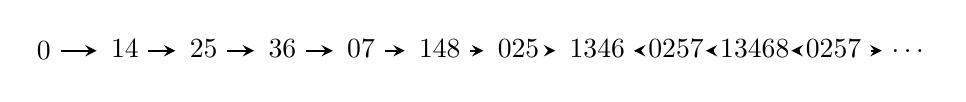
\begin{tikzpicture}[>=stealth, node distance=1cm, every node/.style={sloped}]  % Added slope style for clarity

        % Styles for nodes
        \tikzstyle{state} = []
        
        % Nodes
        \node[state] (0) {0};
        \node[state] (1) [right of=0] {$\begin{matrix} 1 \\ 4 \end{matrix}$};
        \node[state] (2) [right of=1] {$\begin{matrix} 2 \\ 5 \end{matrix}$};
        \node[state] (3) [right of=2] {$\begin{matrix} 3 \\ 6 \end{matrix}$};
        \node[state] (4) [right of=3] {$\begin{matrix} 0 \\ 7 \end{matrix}$};
        \node[state] (5) [right of=4] {$\begin{matrix} 1 \\ 4 \\ 8 \end{matrix}$};
        \node[state] (6) [right of=5] {$\begin{matrix} 0 \\ 2 \\ 5 \end{matrix}$};
        \node[state] (7) [right of=6] {$\begin{matrix} 1 \\ 3 \\ 4 \\ 6 \end{matrix}$};
        \node[state] (8) [right of=7] {$\begin{matrix} 0 \\ 2 \\ 5 \\ 7 \end{matrix}$};
        \node[state] (9) [right of=8] {$\begin{matrix} 1 \\ 3 \\ 4 \\ 6 \\ 8 \end{matrix}$};
        \node[state] (10) [right of=9] {$\begin{matrix} 0 \\ 2 \\ 5 \\ 7 \end{matrix}$};
        \node[state] (11) [right of=10] {\dots};

        % Arrows
        \draw[->, thick] (0) -- (1);
        \draw[->, thick] (1) -- (2);
        \draw[->, thick] (2) -- (3);
        \draw[->, thick] (3) -- (4);
        \draw[->, thick] (4) -- (5);
        \draw[->, thick] (5) -- (6);
        \draw[->, thick] (6) -- (7);
        \draw[->, thick] (7) -- (8);
        \draw[->, thick] (8) -- (9);
        \draw[->, thick] (9) -- (10);
        \draw[->, thick] (10) -- (11);

    
    \end{tikzpicture}
    \caption{sous-classes}
\end{figure}
\end{enumerate}



\begin{exercise}[7.3]
Soit la chaîne de Markov à 10 états $E = \{0, \dots, 9\}$ de matrice de transition :

\[
P =
\begin{pmatrix}
1 & 0 & 0 & 0 & 0 & 0 & 0 & 0 & 0 & 0 \\
0 & \frac{1}{8} & 0 & 0 & \frac{7}{8} & 0 & 0 & 0 & 0 & 0 \\
0 & 0 & 0 & \frac{1}{3} & 0 & 0 & \frac{2}{3} & 0 & 0 & 0 \\
0 & 0 & 0 & 0 & 0 & 0 & 0 & \frac{1}{4} & 0 & \frac{3}{4} \\
\frac{1}{2} & 0 & 0 & 0 & 0 & \frac{1}{2} & 0 & 0 & 0 & 0 \\
0 & \frac{1}{4} & 0 & 0 & \frac{1}{4} & 0 & 0 & \frac{1}{4} & 0 & \frac{1}{4} \\
0 & 0 & \frac{1}{2} & 0 & 0 & 0 & 0 & \frac{1}{2} & 0 & 0 \\
0 & 0 & 0 & 0 & 0 & 0 & 0 & 0 & 1 & 0 \\
\frac{2}{5} & 0 & 0 & 0 & \frac{1}{5} & 0 & 0 & 0 & 0 & \frac{2}{5} \\
0 & 0 & \frac{1}{3} & 0 & 0 & 0 & \frac{1}{3} & 0 & 0 & \frac{1}{3}
\end{pmatrix}.
\]

\begin{enumerate}
    \item \textbf{Tracer son graphe.}
    \item \textbf{Déterminer les classes de la chaîne et leurs périodes.}
\end{enumerate}
\end{exercise}

\subsection*{Solution de l’exercice 7.3}
\begin{enumerate}
    \item Le graphe associé est :

\begin{figure}[h!]
    \centering
    \begin{tikzpicture}[>=stealth, node distance=2cm]

        % Styles for nodes and groups
        \tikzstyle{state} = [circle, draw, fill=red!40, minimum size=0.8cm]
        

        % Nodes
        \node[state] (0) {0};
        \node[state] (5) [right=3cm of 0] {5};
        \node[state] (1) [right=3cm of 5] {1};
        \node[state] (4) [below left=2cm and 1.5cm of 5] {4};
        \node[state] (8) [below left=2cm and 1cm of 1] {8};
        \node[state] (2) [below=5.5cm of 0] {2};
        \node[state] (3) [below=4cm of 5] {3};
        \node[state] (6) [below=2cm of 3] {6};
        \node[state] (7) [below=4cm of 1] {7};
        \node[state] (9) [below=2cm of 7] {9};

       % Groups with custom dimensions
        \node[draw=red, thick, inner sep=0pt, minimum width=2.2cm, minimum height=1.2cm, fit=(0)] {}; 
        
        \node[draw=red, thick, inner sep=0pt, minimum width=6cm, minimum height=2.2cm, fit={(5) (1)}] {};
        
        \node[draw=red, thick, inner sep=0pt, minimum width=6cm, minimum height=2cm, fit={(4) (8)}] {};
        
        \node[draw=red, thick, inner sep=4pt, minimum width=10cm, minimum height=5cm, fit={(2) (3) (6) (7) (9)}] {};


        % Arrows
        \draw[->, thick] (0) edge[loop left] node[left] {1} (0);
        
        \draw[->, thick] (1) edge[loop right] node[right] {$\frac{1}{8}$} (1);
        \draw[->, thick, bend left=25] (5) to node[above] {$\frac{3}{4}$} (1);
        \draw[->, thick, bend left=25] (1) to node[below] {$\frac{7}{8}$} (5);
        \draw[->, thick] (5) edge[loop left] node[left] {$\frac{1}{4}$} (5);
        \draw[->, thick, bend left=25] (4) to node[left] {$\frac{1}{4}$} (5);
        \draw[->, thick, bend left=25] (4) to node[left] {$\frac{1}{2}$} (0);
        \draw[->, thick, bend left=25] (8) to node[right] {$\frac{2}{5}$} (0);
        \draw[->, thick, bend right=25] (8) to node[left] {$\frac{1}{5}$} (5);
    
        \draw[->, thick, bend left=25] (4) to node[above] {$\frac{1}{4}$} (8);
        \draw[->, thick, bend left=25] (8) to node[below] {$\frac{1}{5}$} (4);
        \draw[->, thick] (8) edge[loop right] node[right] {$\frac{1}{5}$} (8);
        

        \draw[->, thick, bend left=25] (2) to node[above] {$\frac{2}{3}$} (6);
        \draw[->, thick, bend left=25] (2) to node[left] {$\frac{1}{3}$} (3);
        \draw[->, thick, bend left=25] (3) to node[above] {$\frac{1}{4}$} (7);
        \draw[->, thick, bend left=25] (6) to node[above] {$\frac{3}{4}$} (9);
        \draw[->, thick, bend left=25] (3) to node[above] {$\frac{3}{4}$} (9);
         \draw[->, thick, bend right=40] (7) to node[below] {\large 1} (2);
        \draw[->, thick, bend left=25] (6) to node[above] {$\frac{1}{4}$} (7);
        \draw[->, thick, bend left=40] (9) to node[below] {\large 1} (2);

    \end{tikzpicture}
\end{figure}



    \item Nous constatons l’existence de 4 classes :
    \begin{itemize}
        \item La classe $\{0\}$, qui est \textbf{fermée} et réduite à un point, formant un état absorbant 0.
        \item La classe $\{1, 5\}$, qui est \textbf{fermée} et \textbf{apériodique}, en raison des boucles en $1$ et $5$.
        \item La classe $\{2, 3, 6, 7, 9\}$, qui est \textbf{fermée} et de \textbf{période 3}. Les 3 sous-classes étant dans l’ordre $\{2\}$, $\{3, 6\}$ et $\{7, 9\}$.
        \item Enfin, la classe $\{4, 8\}$, que nous pouvons quitter vers les classes $\{0\}$ et $\{1, 5\}$, et qui n’est donc pas fermée.
    \end{itemize}

    Nous pouvons voir que nous quittons la classe non fermée $\{4, 8\}$ vers les classes fermées $\{0\}$ et $\{1, 5\}$. Il serait intéressant de savoir avec quelle probabilité nous nous retrouvons dans chacune des deux classes terminales. Or, nous voyons que nous quittons la classe $\{4, 8\}$ de $4$ ou de $8$, et que nous avons toujours deux fois plus de chances de nous retrouver en $0$ que dans la classe $\{1, 5\}$. Par suite, la probabilité de se retrouver en $0$ est $\frac{2}{3}$ et en $\{1, 5\}$ est $\frac{1}{3}$.
\end{enumerate}



\begin{exercise}[7.4]
Déterminer les classes et périodes des exercices suivants du Chapitre 5 :
\begin{itemize}
    \item Exercice 5.4 (marche aléatoire sur $\mathbb{Z}$),
    \item Exercice 5.6 (fort carré),
    \item Exercice 5.7 (transmission d’un bit informatique),
    \item Exercice 5.9 (ruine du joueur),
    \item Exercice 5.10 (plagiste et ses voiliers).
\end{itemize}
\end{exercise}

\subsection*{Solution de l’exercice 7.4}
\begin{itemize}
    \item \textbf{Exercice 5.4 (marche aléatoire sur $\mathbb{Z}$)} : Chaîne irréductible de période 2.
    \item \textbf{Exercice 5.6 (fort carré)} : Chaîne irréductible de période 2, avec comme sous-classes $\{0, 2\}$ et $\{1, 3\}$. De manière générale, la marche aléatoire sur $\mathbb{Z}/n\mathbb{Z}$ est irréductible :
    \begin{itemize}
        \item \textbf{Apériodique} si $n$ est impair,
        \item \textbf{Périodique de période 2} si $n$ est pair.
    \end{itemize}
    \item \textbf{Exercice 5.7 (transmission d’un bit informatique)} : Chaîne irréductible \textbf{apériodique} (car contient des boucles).
    \item \textbf{Exercice 5.9 (ruine du joueur)} : Trois classes :
    \begin{itemize}
        \item $\{0\}$,
        \item $\{N\}$,
        \item $\{1, \dots, N-1\}$.
    \end{itemize}
    Les classes $\{0\}$ et $\{N\}$ consistent en un seul sommet et sont \textbf{fermées}, il s’agit d’états absorbants. La classe $\{1, \dots, N-1\}$ n’est pas fermée, car les classes $\{0\}$ et $\{N\}$ sont accessibles depuis elle. Les deux états absorbants sont de période 1 chacun. La classe non fermée $\{1, \dots, N-1\}$ est de période 2.
    \item \textbf{Exercice 5.10 (plagiste et ses voiliers)} : Chaîne irréductible \textbf{apériodique} (car contient des boucles).
\end{itemize}

\subsection{Récurrence et Transience}

Nous allons étudier une seconde classification des états dépendant du type de comportement de la chaîne. Dans toute cette section, nous considérons une chaîne de Markov $(X_n)_{n \geq 0}$ à valeurs dans un espace $E$, de matrice de transition $P$.
\\
Étant donné un état $x \in E$, tel que $P[X_0 = x] > 0$, nous notons simplement $P_x$ la probabilité conditionnelle 
$P\{  X_0 = x\} $ 
%MASD 
\\ MASD \\
sachant l’événement $\{X_0 = x\}$ réalisé.



\subsubsection{Définitions}

\begin{definition}[7.7]
Soit $x \in E$ un état. Le \textbf{temps d’atteinte} de $x$, noté $T_x$, est le premier instant où $x$ est visité après le départ. Par convention, le temps d’atteinte est infini si nous n’atteignons jamais $x$ :
\[
\forall \omega \in \Omega, \ T_x(\omega) =
\begin{cases}
\inf\{n > 0 \mid X_n(\omega) = x\}, & \text{si un tel entier existe,} \\
+\infty, & \text{sinon.}
\end{cases}
\]
Si la chaîne part de l’état $x$ lui-même, nous employons plutôt le terme de \textbf{temps de retour}.
\end{definition}

\begin{definition}[7.8]
Un état $x \in E$ est dit \textbf{récurrent} si
\[
P_x[T_x < +\infty] = 1.
\]
L’état $x$ est dit \textbf{transient} ou \textbf{transitoire} sinon, c’est-à-dire quand
\[
P_x[T_x < +\infty] < 1, \quad \text{autrement dit } P_x[T_x = +\infty] > 0.
\]
Un état est récurrent si nous sommes sûrs d’y revenir. Il est transient s’il existe une probabilité non nulle de ne jamais y revenir, et donc de le quitter définitivement.
\end{definition}
\subsubsection{Critères de récurrence/transience}

Une manière de caractériser la récurrence/transience d’un état est d’utiliser le nombre de visites, notion que nous introduisons maintenant.

\begin{definition}[7.9]
Le \textbf{nombre de visites} en un état $x$ est la variable aléatoire $N_x$ définie par :
\[
N_x = \sum_{n=0}^{\infty} \mathbf{1}_{\{X_n = x\}}.
\]
La quantité $G(x, y) := \mathbb{E}_x[N_y]$ est l’espérance du nombre de visites en $y$ partant de $x$. $G$ s’appelle le \textbf{noyau de Green}, le \textbf{noyau potentiel} ou simplement la \textbf{fonction de Green}.
\end{definition}

\begin{lemme}[7.10]
Nous avons l’égalité suivante :
\[
\forall (x, y) \in E^2, \ G(x, y) = \sum_{n=0}^{\infty} P^{(n)}(x, y).
\]
\end{lemme}

\begin{demo}
Par définition de la fonction de Green :
\[
G(x, y) = \mathbb{E}_x[N_y] = \mathbb{E}_x \left[\sum_{n \geq 0} \mathbf{1}_{\{X_n = y\}}\right],
\]
(par définition du nombre de visites en $y$)
\[
= \sum_{n \geq 0} \mathbb{E}_x\left[\mathbf{1}_{\{X_n = y\}}\right],
\]
(par inversion de la sommation et de l’espérance, théorème de Fubini)
\[
= \sum_{n \geq 0} P_x[X_n = y],
\]
(espérance de l’indicatrice)
\[
= \sum_{n \geq 0} P^{(n)}(x, y).
\]
\end{demo}


%partie noureediine gajja
\newtheorem{theoreme}{Théorème} 
\begin{theoreme}[7.11]
Les conditions suivantes sont équivalentes :
\begin{enumerate}
    \item L’état \(x \in E\) est récurrent, c'est-à-dire \(P_x[T_x < \infty] = 1\).
    \item \(P_x[N_x = \infty] = 1\).
    \item \(G(x, x) = \infty\).
\end{enumerate}

De manière analogue, les conditions suivantes sont équivalentes :
\begin{enumerate}
    \item L’état \(x \in E\) est transient, c'est-à-dire \(P_x[T_x < \infty] < 1\).
    \item \(P_x[N_x = \infty] = 0\).
    \item \(G(x, x) < \infty\) et \(G(x, x) = \frac{1}{P_x[T_x = \infty]}.\)
\end{enumerate}

Dans ce cas, la loi conditionnelle de \(N_x\) sachant que l’on part de l’état \(x\) est une loi géométrique de paramètre \(P_x[T_x = \infty]\).
\end{theoreme}

Avant de démontrer le Théorème 7.11, nous prouvons le résultat préliminaire suivant :.

\begin{lemme}[7.12]
Pour tout \((x, y) \in E^2\),
\begin{enumerate}
    \item Pour tout \(n \in \mathbb{N}^*\),
    \[
    P_x[N_y \geq n + 1] = P_x[T_y < \infty]P_y[N_y \geq n];
    \]
    cette égalité est aussi vraie pour \(n = 0\) si \(x \neq y\).

    \item Pour la fonction de Green,
    \[
    G(x, y) = \delta_{\{x=y\}} + P_x[T_y < \infty]G(y, y).
    \]
\end{enumerate}
\end{lemme}

\begin{proof}
Démontrons la première égalité. Soit \(n \in \mathbb{N}^*\). D’après la formule des probabilités totales :
\[
P_x[N_y \geq n + 1] = P_x[N_y \geq n + 1, T_y < \infty] + P_x[N_y \geq n + 1, T_y = \infty].
\]
Or, \(P_x[N_y \geq n + 1, T_y = \infty] = 0\), donc :
\[
P_x[N_y \geq n + 1] = P_x[N_y \geq n + 1, T_y < \infty].
\]
Par la formule des probabilités totales :
\[
P_x[N_y \geq n + 1] = \sum_{\ell=1}^\infty P_x[N_y \geq n + 1, T_y = \ell].
\]
En utilisant la définition de \(N_y\) :
\[
P_x[N_y \geq n + 1, T_y = \ell] = P_x\left[\sum_{k=\ell+1}^\infty \mathds{1}_{\{X_k = y\}} \geq n, T_y = \ell \right].
\]
Par les probabilités conditionnelles :
\[
P_x\left[\sum_{k=\ell+1}^\infty \mathds{1}_{\{X_k = y\}} \geq n, T_y = \ell \right] = P\left[\sum_{k=\ell+1}^\infty \mathds{1}_{\{X_k = y\}} \geq n \mid T_y = \ell, X_0 = x \right] P_x[T_y = \ell].
\]

Or, d’après le Corollaire 6.3 :
\[
P\left[\sum_{k=\ell+1}^\infty \mathds{1}_{\{X_k = y\}} \geq n \mid T_y = \ell, X_0 = x \right] = P_y[N_y \geq n].
\]
Ainsi :
\[
P_x[N_y \geq n + 1] = P_y[N_y \geq n] \sum_{\ell=1}^\infty P_x[T_y = \ell].
\]
En conclusion :
\[
P_x[N_y \geq n + 1] = P_y[N_y \geq n]P_x[T_y < \infty].
\]

Démontrons maintenant l’égalité pour la fonction de Green. Par définition :
\[
G(x, y) = \sum_{n=0}^\infty P^{(n)}(x, y).
\]
D’après le Lemme 7.10 :
\[
G(x, y) = \delta_{\{x=y\}} + \sum_{n=1}^\infty P^{(n)}(x, y).
\]
En utilisant la formule des probabilités totales :
\[
P^{(n)}(x, y) = \sum_{\ell=1}^n P_x[X_n = y, T_y = \ell].
\]
Par les probabilités conditionnelles :
\[
P_x[X_n = y, T_y = \ell] = P[X_n = y \mid T_y = \ell, X_0 = x]P_x[T_y = \ell].
\]
D’après le Corollaire 6.3, pour tout \(\ell \in \{1, \dots, n\}\),
\[
P[X_n = y \mid T_y = \ell, X_0 = x] = P_y[X_{n-\ell} = y].
\]
En remplaçant et en inversant les sommes :
\[
G(x, y) = \delta_{\{x=y\}} + \sum_{\ell=1}^\infty P_x[T_y = \ell] \sum_{n=\ell}^\infty P_y[X_{n-\ell} = y].
\]
Or :
\[
\sum_{n=\ell}^\infty P_y[X_{n-\ell} = y] = G(y, y).
\]
Ainsi :
\[
G(x, y) = \delta_{\{x=y\}} + P_x[T_y < \infty]G(y, y).
\]
\end{proof}



\textbf{Démonstration du Théorème 7.11.} Puisque \(P_x[N_x \geq 1] = 1\), le Lemme 7.12 et une récurrence immédiate nous disent que, pour tout \(n \in \mathbb{N}^*\),
\[
P_x[N_x \geq n] = P_x[T_x < \infty]^{n-1}.
\]
La suite d'événements \(\{N_x \geq n\}_{n \geq 1}\) étant décroissante, on a aussi
\[
P_x[N_x = \infty] = P_x\left[\bigcap_{n \geq 1} \{N_x \geq n\}\right] = \lim_{n \to \infty} P_x[N_x \geq n] = \lim_{n \to \infty} P_x[T_x < \infty]^{n-1}.
\]
Ceci montre l'équivalence entre les points 2 et 1. En effet, on a soit
\[
P_x[N_x = \infty] = 1 \Leftrightarrow P_x[T_x < \infty] = 1, \quad \text{ou bien} \quad P_x[N_x = \infty] = 0 \Leftrightarrow P_x[T_x < \infty] < 1.
\]

Montrons maintenant l'équivalence entre les points 1 et 3. D'après la deuxième égalité du Lemme 7.12, la fonction de Green \(G(x, x)\) satisfait à l'égalité
\[
G(x, x)(1 - P_x[T_x < \infty]) = 1.
\]
Ainsi,
\[
G(x, x) = \frac{1}{1 - P_x[T_x < \infty]} < \infty \Leftrightarrow P_x[T_x < \infty] < 1 \quad \text{ou bien} \quad G(x, x) = \infty \Leftrightarrow P_x[T_x < \infty] = 1.
\]
Cela démontre l'équivalence entre le point 1 et le point 3 et termine la preuve des équivalences.

Montrons encore que dans le cas transient, la loi conditionnelle de \(N_x\) sachant \(\{X_0 = x\}\) est géométrique de paramètre \(P_x[T_x = \infty]\). Pour cela, on utilise à nouveau le Lemme 7.12. Pour tout \(n \geq 1\),
\[
P_x[N_x = n] = P_x[N_x \geq n] - P_x[N_x \geq n + 1] = P_x[T_x < \infty]^{n-1} (1 - P_x[T_x < \infty]).
\]

\subsubsection{Classes récurrentes/transientes}
Nous allons établir que la notion de récurrence/transience est une propriété de classes.

\textbf{Proposition 7.13.} Soient deux états \(x\) et \(y\) qui communiquent, alors \(x\) et \(y\) sont soit tous les deux récurrents soit tous les deux transients.

\textbf{Démonstration.} D’après le Théorème 7.11, il suffit de montrer que \(G(x, x)\) et \(G(y, y)\) sont de même nature (soit finies, soit infinies). D’après le Lemme 7.10, pour tout \(x \in E\), on a \(G(x, x) = \sum_{n=0}^{\infty} P^{(n)}(x, x)\), donc cela revient à montrer que les séries de terme général \(P^{(n)}(x, x)\) et \(P^{(n)}(y, y)\) sont de même nature.

Comme \(x\) et \(y\) communiquent, il existe \(k, \ell\) tels que \(P^{(k)}(x, y) > 0\) et \(P^{(\ell)}(y, x) > 0\). Ainsi, for everything \(n \geq k + \ell\), \[ P^{(n)}(x, x) \geq P^{(k)}(x, y) P^{(n-k-\ell)}(y, y) P^{(\ell)}(y, x) \] and \[ P^{(n)}(y, y) \geq P^{(\ell)}(y, x) P^{(n-k-\ell)}(x, x) P^{(k)}(x, y), \] it is this that shows that the two séries converge and divergent in the same time.
\textbf{Définition 7.14.} Une classe d’équivalence est dite récurrente, resp. transiente, si un de ses sommets est récurrent, resp. transient.

\textbf{Proposition 7.15.} Une classe récurrente est fermée, autrement dit, la probabilité de sortir d’une classe récurrente est nulle.

\textbf{Démonstration.} Soit \(x\) un état quelconque appartenant à la classe de récurrence \(C\). Supposons qu’il existe \(y \notin C\) tel que \(x \to y\) et montrons que cela conduit à une contradiction. Remarquons d’abord que \(y\) ne conduit à aucun sommet de \(C\), car sinon on aurait \(y \to x\), donc \(x \leftrightarrow y\), et \(y \in C\). De plus, on a :
\[
x \to y \iff P_x[T_y < \infty] > 0.
\]
Or, la probabilité \(P_x[T_x = \infty]\) de ne pas revenir en \(x\) est bornée inférieurement par la probabilité d’aller en \(y\) en temps fini (puisque \(y\) ne conduit à aucun état de \(C\)). Ainsi,
\[
P_x[T_x = \infty] \geq P_x[T_y < \infty] > 0,
\]
ce qui donne \(P_x[T_x < \infty] < 1\), ce qui est une contradiction avec le fait que \(x\) est récurrent. 
Nous voyons qu’une classe récurrente est fermée, mais la réciproque est fausse en général (voir l’exemple de la marche aléatoire non-symétrique, Exercice 7.7, qui est fermée et transiente), bien que cette réciproque soit vérifiée si cette classe est de cardinal fini.

\textbf{Proposition 7.16.} Toute classe fermée et de cardinal fini est récurrente.

\textbf{Démonstration.} Soit \(C\) cette classe fermée, et soit \(x \in C\), alors,
\[
\sum_{y \in C} G(x, y) = \sum_{y \in C} \sum_{n \geq 0} P^{(n)}(x, y) = \sum_{n \geq 0} \sum_{y \in C} P^{(n)}(x, y) = \infty,
\]
car pour tout \(n \in \mathbb{N}\),
\[
\sum_{y \in C} P^{(n)}(x, y) = P_x[X_n \in C] = 1 ; \text{ puisque la classe } C \text{ est fermée, nous ne la quittons pas.}
\]
Supposons que pour tout \(y \in C\), \(y\) soit transient. Alors d’après l’Exercice 7.5, \(G(x, y) < \infty\). Par hypothèse, la classe \(C\) est de cardinal fini, ce qui implique que \(\sum_{y \in C} G(x, y) < \infty\), et cela donne une contradiction. En conséquence, il existe un état \(y \in C\) récurrent et la classe \(C\) est donc récurrente.

\textbf{Corollaire 7.17.} Une chaîne de Markov définie sur un espace d’états fini admet au moins un état récurrent.

\textbf{Démonstration.} Ceci découle du fait que si l’espace d’état est fini, il doit y avoir au moins une classe fermée.






\newpage

\subsection{Exercices : récurrence/transience}
\vspace{5mm}
\textbf{Exercice 7.5} [Fonction de Green]

\noindent Allons un peu plus loin dans l’étude de la fonction de Green. Soit $x, y \in E$ deux états. Montrer que :
\begin{enumerate}
    \item Si $x \not\to y$, alors $G(x, y) = 0$.
    \item Si $x \to y$ et
    \begin{itemize}
        \item $y$ est transient, alors $G(x, y) < \infty$ ;
        \item $y$ est récurrent, alors $G(x, y) = \infty$.
    \end{itemize}
    \item La fonction de Green satisfait à l'équation,
    \[
    G = PG + I \quad \Leftrightarrow \quad \forall (x, y) \in E^2, \, G(x, y) = \sum_{z \in E} p(x, z)G(z, y) + \delta_{\{x=y\}}.
    \]
\end{enumerate}

\noindent \textit{Solution de l’exercice 7.5.}\\
\begin{enumerate}
    \item Si \(x \not\to y\), alors pour tout \(n \geq 0, P^{(n)}(x, y) = 0\). Ainsi, d’après le Lemme 7.10, \(G(x, y) = 0\).
    \item On a,
    \[
    x \to y \quad \Leftrightarrow \quad \mathbb{P}_x [T_y < \infty] > 0,
    \]
    (Preuve dans l’Exercice 9.6. de “Exercices de Probabilités”, Cottrell \& al.)\\
    De plus, si y est transient, \(G(y, y) < \infty\) et si \(y\) est récurrent \(G(y, y) = \infty\). En utilisant la deuxième égalité du Lemme 7.12, ceci démontre le point 2.
    \item D’après le Lemme 7.10,
    \begin{align*}
        G(x, y) &= \sum_{n=0}^\infty P^{(n)}(x, y) = P^{(0)}(x, y) + \sum_{n=1}^\infty P^{(n)}(x, y) \\
        &= \delta_{\{x=y\}} + \sum_{n=1}^\infty \sum_{z \in E} p(x, z) P^{(n-1)}(z, y), \quad \text{d'après Chapman-Kolmogorov} \\
        &= \delta_{\{x=y\}} + \sum_{z \in E} p(x, z) \sum_{n=1}^\infty P^{(n-1)}(z, y) = \delta_{\{x=y\}} + \sum_{z \in E} p(x, z) \sum_{n=0}^\infty P^{(n)}(z, y) \\
        &= \delta_{\{x=y\}} + \sum_{z \in E} p(x, z) G(z, y).
    \end{align*}
\end{enumerate}


\noindent\textbf{Exercice 7.6.}
On considère une chaîne de Markov $(X_n)_{n \geq 0}$ d’espace d’état $E = \{1, 2, 3\}$ et de matrice de transition 
\[
P = 
\begin{pmatrix}
0 & 1 & 0 \\
\frac{1}{2} & \frac{1}{2} & 0 \\
\frac{1}{3} & \frac{1}{3} & \frac{1}{3}
\end{pmatrix}.
\]

\begin{enumerate}
    \item Dessiner le graphe associé à cette chaîne de Markov et classifier les états (récurrents/transients).
    \item Calculer la fonction de Green pour toutes les paires de points $(x, y) \in E^2$. En déduire la probabilité de ne jamais revenir en $3$ sachant que l’on est parti de $3$.
\end{enumerate}

\noindent \textit{Solution de l’exercice 7.6.}\\
\begin{enumerate}
    \item Graphe à faire. Les classes d’équivalence sont ${1, 2}$ et ${3}$. La classe ${1, 2}$ est fermée et finie, donc récurrente. La classe ${3}$ permet d’atteindre la classe ${1, 2}$ ; elle n’est pas fermée, donc transiente.
    \item  D’après les points $1$ et $2$ de l’Exercice 7.5, on a que la matrice des coefficients de la fonction de Green est de la forme,

    \[
    G = 
    \begin{pmatrix}
        \infty & \infty & 0 \\
        \infty & \infty & 0 \\
        \infty & \infty & G(3, 3)
    \end{pmatrix}
    \]
\end{enumerate}
\noindent Pour déterminer $G(3, 3)$ on utilise le Point 3 de l’Exercice 7.5 :
\[
G(3, 3) = 1 + \sum^{3}_{z=1}p(z, 3)G(z, 3) = 1 + \frac{1}{3}G(3, 3).
\]

\noindent Ainsi, $\frac{2}{3}G(3, 3) = 1$, autrement dit $G(3, 3) = \frac{3}{2}$. On en déduit la probabilité de ne jamais revenir en $3$ sachant que l’on est parti de $3$ :
\[
\mathbb{P}_3[T_3 = \infty] = \frac{1}{G(3, 3)} = \frac{2}{3}
\]


\noindent \textbf{Exercice 7.7} Classifier les états (récurrents / transients) des exercices du Chapitre 5.3 : Exercice 5.4 (marche aléatoire sur $\mathbb{Z}$), Exercice 5.6 (fort carré), Exercice 5.7 (transmission d’un bit informatique), Exercice 5.9 (ruine du joueur), Exercice 5.10 (plagiste et ses voiliers).\\

\noindent \textit{Solution de l’exercice 7.7.}
\begin{itemize}
    \item Exercice 5.4 (marche aléatoire sur $\mathbb{Z}$). Chaîne irréductible. Il suffit donc de considérer un état. Dans l’Exercice 6.4 on a montré que
\[
\text{Si} \quad p \neq \frac{1}{2}, G(x, x) = \sum_{n=0}^{\infty}P^{(n)}(x,x) < \infty
\]
\[
\text{Si} \quad p = \frac{1}{2}, G(x, x) = \sum^{\infty}_{n=0}P^{(n)}(x, x) = \infty
\]

\noindent Ainsi, la marche aléatoire est récurrente dans le cas symétrique et transiente sinon. Remarquer que dans le cas non symétrique, on a un exemple de classe fermée (infinie) et non-récurrente.
    \item Exercice 5.6 (fort carré) ou marche aléatoire sur $\mathbb{Z}/n\mathbb{Z}$.Chaîne irréductible. Elle est récurrente car finie.
    \item Exercice 5.7 (transmission d’un bit informatique). Chaîne irréductible. Elle est récurrente car finie.
    \item Exercice 5.9 (ruine du joueur). Trois classes : $\{0\}, \{N\}, \{1,..., N-1\}$  Les classes $\{0\}, \{N\}$ consistent en un seul sommet et sont fermées, il s’agit d’états absorbants. La classe $\{1,..., N-1\}$ n’est pas fermée car les classes $\{0\}, \{N\}$ sont accessibles depuis elle. Ainsi les états absorbants sont récurrents et la classe $\{1,..., N-1\}$ est transiente.
    \item Exercice 5.10 (plagiste et ses voiliers). Chaîne irréductible. Elle est récurrente car finie.
\end{itemize}

\noindent \textbf{Exercice 7.8 [Qui perd, perd tout]}

Nous considérons un joueur dont la probabilité de donner une bonne réponse est $p$ quelle que soit la question posée et la probabilité de donner une réponse fausse est $1-p$, avec $0 < p < 1$. Nous supposons que les réponses sont indépendantes les unes des autres et que s’il donne une bonne réponse, il gagne 1, et s’il donne une mauvaise réponse, il perd tout. La richesse de départ est $X_0 = 0$ et, pour tout $n \geq 1$, on note $X_n$ sa fortune à l’instant $n$.
\begin{enumerate}
    \item Montrer qu’il s’agit d’une chaîne de Markov. Donner son graphe et sa matrice de transition.
    \item Montrer que cette chaîne de Markov est irréductible.
    \item Soit $T_0 = \inf\{n > 0 \mid X_n = 0\}$ le temps d’atteinte de $0$. Pour tout $n \in \mathbb{N}^*$, calculer $P_0[T_0 = n]$.
    \item En déduire que la chaîne est récurrente.
\end{enumerate}

\noindent \textit{Solution de l’exercice 7.8.}
\begin{enumerate} 
    \item Le processus $(X_n)_{n \geq 0}$ est à valeurs dans $E = \mathbb{N}$. Soit $Y_n$ la variable aléatoire valant 1 si le joueur répond juste à la n-ième question, et 0 sinon. Alors $(Y_n)_{n\geq 1}$ est une suite de variables aléatoires i.i.d. de loi de Bernoulli de paramètre $p$, indépendante de $X_0$. Pour tout $n \geq 0$, la fortune du joueur à l’instant $n + 1$ est :

\[
X_{n+1} = 
\begin{cases}
X_n + 1 & \text{si } Y_{n+1} = 1 \\
0 & \text{si } Y_{n+1} = 0
\end{cases}
\]
\[
= (X_n + 1) \mathbb{I}_{\{Y_{n+1}=1\}}.
\]
Ainsi d’après l’Exercice 5.5,$ (X_n)_{n \geq 0}$ est une chaîne de Markov.
La matrice de transition $P = (p(x, y))$ a pour coefficients non nuls,
\[
\forall x \in \mathbb{N}, p(x, x+1) = p \quad p(x, 0) = 1 - p.
\]
\newpage
\begin{figure}[h]
\[
P =
\begin{array}{c@{}c@{}c} 
\begin{array}{r}
0 \quad 1 \quad 2 \quad 3 \quad \cdots
\end{array}
\\
\begin{pmatrix}
    1 - p & p & 0 & 0 & \cdots \\
    1 - p & 0 & p & 0 & \cdots \\
    1 - p & 0 & 0 & p & \cdots \\
    1 - p & 0 & 0 & 0 & \cdots \\
    \vdots & \vdots & \vdots & \vdots & \ddots
\end{pmatrix}
&
\begin{array}{r}
0 \\ 1 \\ 2 \\ 3 \\ \vdots
\end{array}

\end{array}
\]
\centering
\caption{Matrice de transition du jeu.}
\end{figure}


\noindent Le graphe associé à cette chaîne de Markov est,
\begin{figure}[h!]
    \centering
    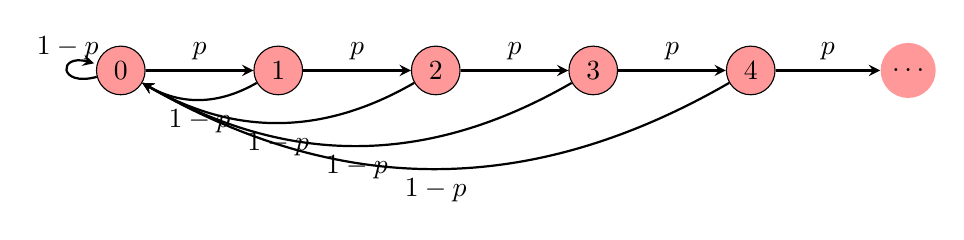
\begin{tikzpicture}[>=stealth, node distance=2cm]
        % Style des noeuds
        \tikzstyle{state} = [circle, draw, fill=red!40, minimum size=0.5cm, node distance=2cm]

        % Définition des noeuds
        \node[state] (0) {0};
        \node[state] (1) [right of=0] {1};
        \node[state] (2) [right of=1] {2};
        \node[state] (3) [right of=2] {3};
        \node[state] (4) [right of=3] {4};
        \node[state, draw=none] (dots) [right of=4] {$\dots$};

        % Arcs entre les noeuds
        \draw[->, thick] (0) edge[loop left] node[above] {$1-p$} (0);
        \draw[->, thick] (0) -- node[above] {$p$} (1);
        \draw[->, thick] (1) -- node[above] {$p$} (2);
        \draw[->, thick] (2) -- node[above] {$p$} (3);
        \draw[->, thick] (3) -- node[above] {$p$} (4);
        \draw[->, thick] (4) -- node[above] {$p$} (dots);
        
        % Backward arrows
        \draw[->, thick, bend left] (1) to node[below] {$1-p$} (0);
        \draw[->, thick, bend left] (2) to node[below] {$1-p$} (0);
        \draw[->, thick, bend left] (3) to node[below] {$1-p$} (0);
        \draw[->, thick, bend left] (4) to node[below] {$1-p$} (0);

    \end{tikzpicture}
    \caption{Graphe de la ruine du joueur.}
\end{figure}

    \item Nous constatons que tous les points communiquent entre eux. En effet, soient deux états $x$ et $y$ :
    \begin{itemize}
        \item Si $y > x$, alors partant de $x$ nous pouvons atteindre $y$ en $y - x$ étapes en gagnant successivement $y - x$ fois : $P^{(x - y)}(x, y) = p^{y - x} > 0$.

        \item Si $y<x$, alors partant de x nous pouvons perdre immédiatement et gagner $y$ fois pour atteindre la fortune $y: P^{(1+y)}(x, y) = (1-p)p^y > 0$.
    \end{itemize}
Il n’y a donc qu’une seule classe et la chaîne est irréductible.\\
\item Soit $n \in \mathbb{N}^*$. Alors,\\

\begin{align*}
    \mathbb{P}_0[T_0=n] &= \mathbb{P}[\{\text{le joueur répond juste aux $(n-1)$ premières questions et faux à la n-ième\}}] \\
    &= \mathbb{P}_0[\{Y_1 = 1, \dots, Y_n-1 = 1, Y_n = 0\}], \text{ d'après Chapman-Kolmogorov} \\
    &= p^{n-1}(1-p), \text{ par indépendance} \\ 
\end{align*}


Ainsi la loi conditionnelle de $T_0$ sachant ${X_0 = 0}$ est une loi géométrique de paramètre $(1-p)$ sur $N^*$

\item On a, 
$$
\mathbb{P}_0[T_0 < \infty] = \sum^{\infty}_{n=1}\mathbb{P}_0[T_0=n] = (1-p)\sum^{\infty}_{n=1}p = \frac{1-p}{1-p} = 1
$$
et la chaîne est donc récurrente.
\end{enumerate}


\noindent \textbf{Exercice 7.9 [Ruine du joueur, suite]}

On reprend l’Exercice 5.9 de la ruine du joueur : deux joueurs $A$ et $B$ disposent d’une fortune initiale de $a$ et $b$ euros respectivement, avec $a, b > 0$. Ils jouent au jeu de hasard suivant : la mise est de 1 euro par partie ; les parties sont indépendantes et à chacune d’entre elles le joueur $A$ a une probabilité $p$ de gagner (et donc $1-p$ de perdre), avec $0 < p < 1$. Le jeu se déroule jusqu’à la ruine d’un des deux joueurs. Notons $N = a + b$, alors la durée du jeu est $T = \inf\{n > 0 \mid X_n \in \{0, N\}\}$. Calculer la probabilité que le joueur $A$ gagne.\\


\noindent \textit{Solution de l’exercice 7.9.} Notons $u(x) = P_x[X_T = N]$, c’est-à-dire la probabilité que le joueur gagne sachant que sa fortune initiale est $x$, avec $x \in \{0, \dots , N\}$. Finalement, on sera intéressé par la probabilité $u(a)$ mais on verra qu’il est utile d’élargir le problème pour le résoudre.\\
Montrons que pour tout $x \in \{1, \dots , N-1\}$, en écrivant $q = 1-p$, $u(x)$ satisfait à l’équation :
$$u(x) = pu(x + 1) + qu(x - 1).$$
En effet, comme $a, b > 0$, on sait que $T \geq 1$. En décomposant sur toutes les valeurs possibles de\\
la chaîne à l’instant 1, on obtient,
\begin{align*}
    u(x) &= \mathbb{P}_x[X_T = N] = \sum_{y \in E} \mathbb{P}_x[X_T = N \mid X_1 = y] \mathbb{P}_x[X_1 = y] \\
    &= \sum_{y \in E} \mathbb{P}_y[X_T = N] \mathbb{P}_x[X_1 = y], \quad \text{(en utilisant la propriété de Markov)} \\
    &= pu(x + 1) + (1-p)u(x-1), \quad \text{(car les autres termes où } \mathbb{P}_x[X_1 = y] = p(x, y) 
    \text{ sont nuls).}
\end{align*}

On a les conditions au bord suivantes,
$$
u(0) = 0, \quad u(N) = 1.
$$

Il s’agit de résoudre une récurrence linéaire d’ordre 2. L’équation caractéristique est :
$$
pz^2 - z + q = 
$$

Ce polynôme a deux racines $z_{1, 2} = 1$, $\frac{p}{q}$ si $p \neq q$ et une racine double $Z_1 = 1$ si $p = q = \frac{1}{2}$. Ainsi,

\begin{itemize}
    \item Si $p \neq q$, la solution générale est de la forme
    $$
    u(x) = \lambda z_1^x + \mu z_2^x = \lambda + \mu(\frac{q}{p})^x.
    $$
    En tenant compte des conditions initiales, on résout pour $\lambda$, $\mu$ et on trouve,
    $$
    u(x) = \frac{1-(\frac{q}{p})^x}{1-(\frac{q}{p})^N}.
    $$

    \item Si $p = q = \frac{1}{2}$, la solution générale est de la for
    $$
    u(x) = (\lambda + \mu x)z^x_1 = (\lambda + \mu x).
    $$
    En tenant compte des conditions initiales, on résout pour $\lambda$, $\mu$ et on trouve,
    $$
    u(x) = \frac{x}{N}.
    $$
\end{itemize}